\documentclass[12pt,letterpaper]{article}
\usepackage[utf8]{inputenc}
\usepackage{amsmath}
\usepackage{amsfonts}
\usepackage{amssymb}
\usepackage{amsthm}
\usepackage{graphicx}
\usepackage{tabularx}
\usepackage[left=2cm,right=2cm,top=2cm,bottom=2cm]{geometry}
\usepackage{multicol}
\usepackage{listings}
\lstset{ 
basicstyle = \ttfamily,
showstringspaces=false,
upquote=true,
columns=fullflexible,
literate={*}{{\char42}}1
         {-}{{\char45}}1
         {"}{{\fontencoding{T1}\selectfont\textquotedbl}}1
         {'}{{\fontencoding{T1}\selectfont\textquotesingle}}1
}
\usepackage{lastpage}
\usepackage{fancyhdr}
\usepackage{multirow,array}
\usepackage{newtxtext,newtxmath}
\usepackage{lastpage}
\usepackage{enumitem}
\newcolumntype{Y}{>{\centering\arraybackslash}X}
\pagestyle{fancy}
\fancyhf{}
\lhead{\textsc{BHCC Mat-181}}
\chead{\textsc{Answers}}
\rhead{\textsc{HW Exercises 3.17-3.18}}
\rfoot{Page \thepage ~of \pageref{LastPage}}
\setenumerate[1]{label={\bf 3.\theenumi: }}
\setenumerate[2]{label={\bf (\theenumii): }}
\setenumerate[3]{label={\bf \theenumiii: }}

\begin{document}
\newcommand{\N}[2]{\mathcal{N}\big(#1,~#2\big)}
\newcommand{\AND}{\textsc{~and~}}
\newcommand{\OR}{\textsc{~or~}}

\begin{enumerate}
\setcounter{enumi}{16}
\item \begin{enumerate}
\item Let's consider the exam scores corresponding to integer $z$ scores.
\begin{center}
\begin{tabular}{c c c c c c c c c}
$z = $ & -3 & -2 & -1 & 0 & 1 & 2 & 3 \\
$x = $ &52.38 & 60.82 & 69.26 & 77.70 & 86.14 & 94.58 & 103.02
\end{tabular}
\end{center}
There are 14 scores between 69.26 and 86.14. There are 19 scores between 60.82 and 94.58. There are 20 scores between 52.38 and 103.02.
\begin{align*}
\frac{14}{20} &= 0.7 \approx 0.68 \\\\
\frac{19}{20} &= 0.95 = 0.95\\\\
\frac{20}{20} &= 1.0 \approx 0.997
\end{align*}
The exam scores closely match the 68-95-99.7 rule.

\item Yeah. The normal curve matches closely to the histogram, and the Q–Q (quantile-quantile) plot looks nearly linear. Also the 68-95-99.7 analysis suggests normality.
\end{enumerate}

\item \begin{enumerate}
\item Let's consider the heights corresponding to integer $z$ scores.
\begin{center}
\begin{tabular}{c c c c c c c c c}
$z = $ & -3 & -2 & -1 & 0 & 1 & 2 & 3 \\
$x = $ & 47.78 & 52.36 & 56.94 & 61.52 & 66.1 & 70.68 & 75.26
\end{tabular}
\end{center}
There are 17 heights between 56.94 and 66.1. There are 19 heights between 52.36 and 70.68. There are 20 heights between 47.78 and 75.26.
\begin{align*}
\frac{17}{20} &= 0.85 \\\\
\frac{19}{20} &= 0.95\\\\
\frac{20}{20} &= 1.0
\end{align*}

I'm not sure how closely we really expect such a small sample to match the 68-95-99.7 rule. Let's run some simulations.

In R, I can run the command \texttt{sum(abs(rnorm(20))<1)} to run a single simulation of drawing 20 normal random variable and counting how many are within 1 standard deviation. I've repeated this 10 times...

\begin{verbatim}
> sum(abs(rnorm(20))<1)
[1] 15
> sum(abs(rnorm(20))<1)
[1] 14
> sum(abs(rnorm(20))<1)
[1] 17
> sum(abs(rnorm(20))<1)
[1] 13
> sum(abs(rnorm(20))<1)
[1] 16
> sum(abs(rnorm(20))<1)
[1] 15
> sum(abs(rnorm(20))<1)
[1] 11
> sum(abs(rnorm(20))<1)
[1] 12
> sum(abs(rnorm(20))<1)
[1] 12
> sum(abs(rnorm(20))<1)
[1] 18
\end{verbatim}

I can repeat this 10000 times, where each time I sample 20 random normal variables and count how many are outside 1 standard deviation from the mean.
\begin{center}
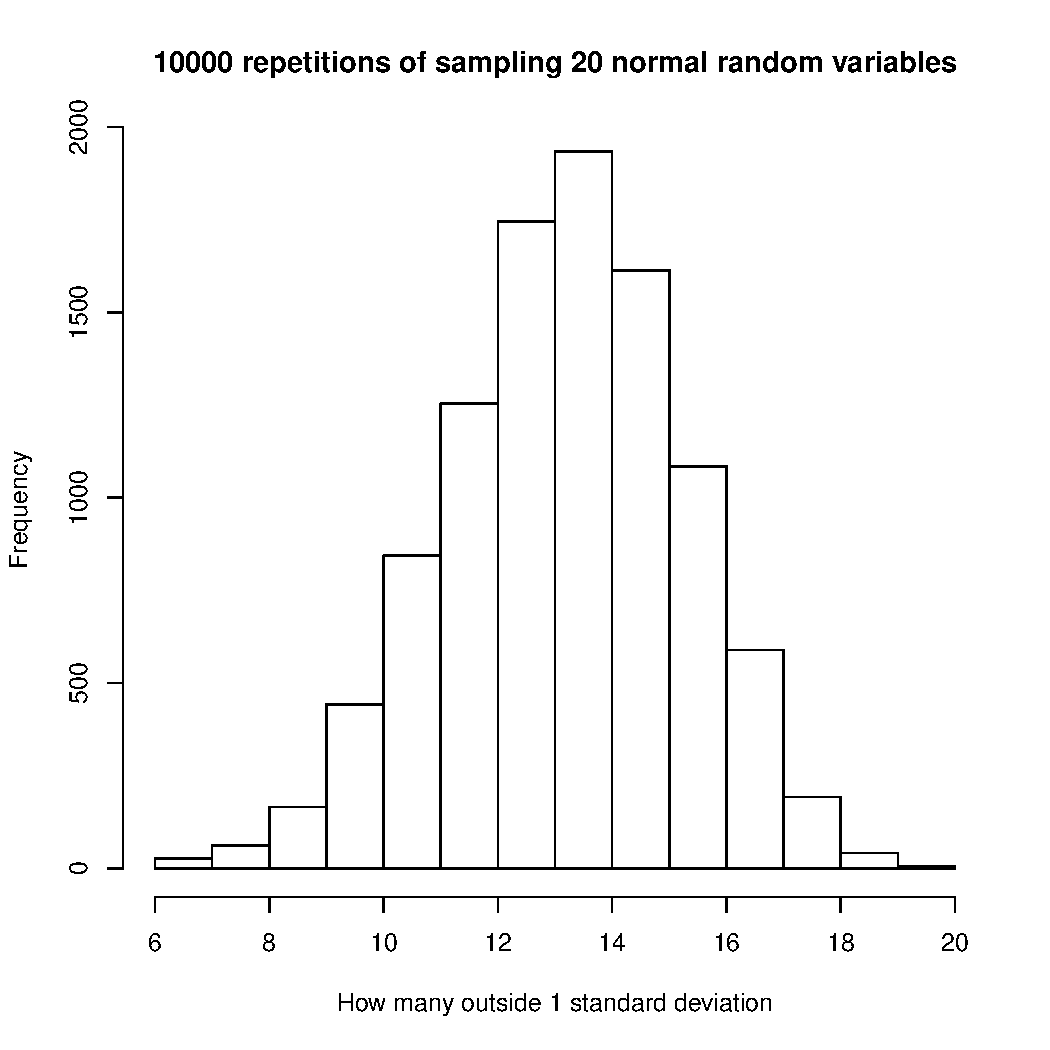
\includegraphics[scale=0.6]{figures/variability_of_68_rule/variability_of_68_rule.pdf}
\end{center}
So, getting 17 (out of 20) within 1 standard deviation (from the mean) seems uncommon but not rare when sampling from a normal distribution.

\newpage
If you are interested, here is the code I ran in R:

\begin{lstlisting}[language=r]
counts = c()
for (i in seq(1,10000))
{
    counts = c(counts,sum(abs(rnorm(20))<1))
}
hist(counts, 
     xlab='How many outside 1 standard deviation',
     main='10000 repetitions of sampling 20 normal random variables')
\end{lstlisting}
\item These data seem like they could be from a normal distribution. There are hints that maybe these data come from a right-skew distribution, but with such a small sample size it is really hard to say anything definitive.
\end{enumerate}

\end{enumerate}
\end{document}
